\lhead[\thepage]{CAPÍTULO \thechapter. VERIFICACIÓN, VALIDACIÓN Y EVALUACIÓN}
\chead[]{}
\rhead[WepSIM: Simulador de procesador elemental con unidad de control microprogramada\leftmark]{\thepage}
\renewcommand{\headrulewidth}{0.5pt}

\lfoot[]{}
\cfoot[]{}
\rfoot[]{}
\renewcommand{\footrulewidth}{0pt}

%% This is an example first chapter.  You should put chapter/appendix that you
%% write into a separate file, and add a line \include{yourfilename} to
%% main.tex, where `yourfilename.tex' is the name of the chapter/appendix file.
%% You can process specific files by typing their names in at the 
%% \files=
%% prompt when you run the file main.tex through LaTeX.
\chapter{Verificación, validación y evaluación}
\label{ch:verification_validation_and_evaluation}
\markboth{}{VERIFICACIÓN, VALIDACIÓN Y EVALUACIÓN}


Este capítulo detalla la verificación, validación y evaluación del proyecto. En primer lugar, presentamos la verificación y validación del simulador (Sección \ref{sec:verification_and_validation}, \textit{\nameref{sec:verification_and_validation}}), y detallamos una serie de pruebas que nos permitieron verificar que habíamos cumplido todos los requisitos establecidos en el Capítulo  \ref{ch:analysis}(\textit{\nameref{ch:analysis}}). Después de esto, mostramos la validación de los resultados de las simulaciones, demostrando que el simulador realiza simulaciones precisas y realistas.

Para la realización de las simulaciones, hemos tomado la definición de un juego de instrucciones base proporcionado por el coordinador de la asignatura Estructura de Computadores, pudiendo así validar que el funcionamiento del simulador es correcto al obtener los resultados esperados en cada una de las instrucciones y códigos simulados en la herramienta. 

\section{Verificación y validación}
\label{sec:verification_and_validation}

El principal objetivo de esta sección es verificar que todos los requisitos detallados en el Capítulo \ref{ch:analysis} (\textit{\nameref{ch:analysis}}) han sido cumplidos. Además, validamos los resultados obtenidos con WepSIM, comparándolos con los resultados teóricos esperados de la definición del juego de instrucciones de la asignatura Estructura de Computadores y los ejercicios especificados en el libro \cite{perez2015problemas}.


En la ingeniería de software, la verificación y validación son los procesos de comprobar que un sistema de software cumple con las especificaciones y que cumple con su propósito. Como se explica en el Capítulo \ref{ch:analysis} (\textit{\nameref{ch:analysis}}), el cliente fija inicialmente los requisitos deseados para el producto final (requisitos del usuario). A partir de ahí, los analistas especifican los requisitos de software (requisitos funcionales y no funcionales). Para verificar que se cumplen los requisitos del proyecto, se necesitan procesos de verificación y validación (ver Figura \ref{fig:verification_validation}).

\vspace{1cm}

\begin{figure}[htb]
 	\centering
 	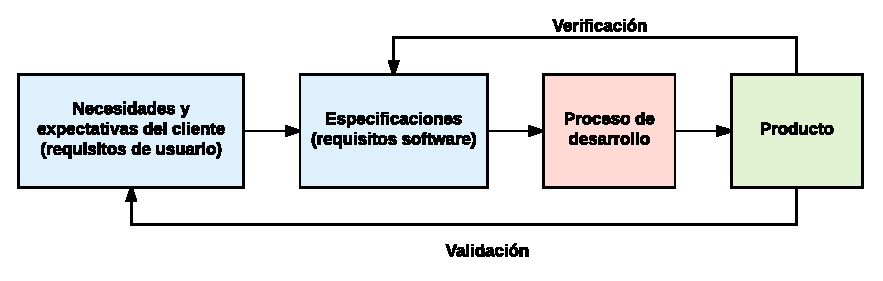
\includegraphics[width=12cm]{figures/verificacion_validacion_diagrama}
 	\caption{Verificación y validación software.}
	\label{fig:verification_validation}
\end{figure}

\vspace{1cm}

\textit{Verificación Software} Es el proceso de evaluación de los productos de trabajo (no el producto final real) de una fase de desarrollo para determinar si cumplen con los requisitos especificados para esa fase (los requisitos de software). \textit{Validación software} es el proceso de evaluación del producto final al final del proceso de desarrollo para determinar si satisface los requisitos especificados por el usuario al inicio del proyecto \cite{verification}.

\subsection{Pruebas de verificación}

Con el fin de realizar las pruebas de verificación, hemos seguido un proceso dinámico durante la fase de desarrollo del software. Con estas pruebas queríamos responder a la pregunta: "¿Estamos construyendo el producto correctamente?". La tabla \ref{tab:verification_tests} proporciona la plantilla utilizada para los test de verificación. Tenga en cuenta que el formato del atributo ID es VET-XX, donde XX indica el número de test de verificación.
\clearpage

\begin{center}
\begin{table*}[htb]
\centering
\begin{tabular}{@{}p{2.5cm} p{9cm}@{}} 
\toprule
\textbf{ID} 					& Test ID. \\
\midrule
\textbf{Nombre} 				& Nombre del test. \\
\midrule
\textbf{Requisitos} 		& Requisitos de software cumplidos con este test. \\
\midrule
\textbf{Descripción} 		& Descripción del test. \\
\midrule
\textbf{Precondiciones}		& Las condiciones que siempre deben ser verdad antes de realizar el test. \\
\midrule
\textbf{Procedimiento}			& Una secuencia fija, paso a paso, de las actividades realizadas por el test. \\
\midrule
\textbf{Postcondiciones} 		& Las condiciones que siempre deben ser verdaderas justo después de realizar el test. \\
\midrule
\textbf{Evaluación} 			& \textit{OK} or \textit{Error}. \\
\bottomrule
\end{tabular}
\caption{Plantilla de pruebas de verificación.}
\label{tab:verification_tests}
\end{table*}
\end{center}

Luego, especificamos las pruebas de verificación.

\vspace{0.7cm}

\begin{center}
\begin{table*}[htb]
\centering
\begin{tabular}{@{}p{2.5cm} p{13cm}@{}} 
\toprule
\textbf{ID} 					& VET-01. \\
\midrule
\textbf{Nombre} 				& Plataforma. \\
\midrule
\textbf{Requisitos} 		& . \\
\midrule
\textbf{Descripción} 		& Verificar que el software puede ser utilizado y ha sido desarrollado con las herramientas especificadas en los requisitos. \\
\midrule
\textbf{Precondiciones}		& 1.Utilizar una máquina con sistema operativo Ubuntu 16.04 / Windows 10 / MacOS 10.2.5 .\\
							& 2. . \\
							& 3. . \\
\midrule
\textbf{Procedimiento}			& 1. . \\
							& 2. .\\
							& 3. .\\
\midrule
\textbf{Postcondiciones} 		& 1. .\\
							& 2. .\\
							& 3. . \\			
							& 4. . \\
\midrule
\textbf{Evaluación} 			& OK \\
\bottomrule
\end{tabular}
\caption{Test de verificación VET-01.}
\label{tab:vet01}
\end{table*}
\end{center}


\begin{center}
\begin{table*}[htb]
\centering
\begin{tabular}{@{}p{2.5cm} p{13cm}@{}} 
\toprule
\textbf{ID} 					& VET-01 \\
\midrule
\textbf{Name} 				& Plataforma. \\
\midrule
\textbf{Requirements} 		& . \\
\midrule
\textbf{Description} 		& Verificar que el sofware puede ser utilizado y ha sido desarrollado con las herramientas especificadas en los requisitos. \\
\midrule
\textbf{Preconditions}		& 1. Use a machine with Ubuntu 14.04 operating system.\\
							& 2. GCC (GNU Compiler) 5.1 or higher must be installed on the machine. \\
							& 3. The user must be located in the main directory of the \gls{comsimboinc} application. \\
\midrule
\textbf{Procedure}			& 1. Check the code of the simulator source files (all these files are inside the /Files folder). \\
							& 2. Run the generator script with the default parameters to create the simulation files.\\
							& 3. Run the simulation.\\
\midrule
\textbf{Postconditions} 		& 1. All source files must be written in C programming language.\\
							& 2. The implementation, setup and control of the simulations must be carried out using the MSG API of the SimGrid toolkit.\\
							& 3. Simulations run while a progress bar indicates the percentage of execution. \\			
							& 4. The simulator must successfully finish its execution in the specified operating system. \\
\midrule
\textbf{Evaluation} 			& Passed \\
\bottomrule
\end{tabular}
\caption{Verification test VET-01.}
\label{tab:vet01}
\end{table*}
\end{center}


\begin{center}
\begin{table*}[htb]
\centering
\begin{tabular}{@{}p{2.5cm} p{13cm}@{}} 
\toprule
\textbf{ID} 					& VET-02 \\
\midrule
\textbf{Name} 				& Realistic BOINC elements in simulations. \\
\midrule
\textbf{Requirements} 		& SR-F-F06, SR-NF-UI01, SR-NF-UI02. \\
\midrule
\textbf{Description} 		& Verify that the simulator allows to simulate all the BOINC actual elements. \\
\midrule
\textbf{Preconditions}		& 1. The user must be located in the main directory of the \gls{comsimboinc} application.\\
\midrule
\textbf{Procedure}			& 1. Specify the following elements in the simulation parameters: tasks, volunteer hosts, servers, data servers, networks, and hosts availability.\\
							& 2. Run the generator script to create the simulation files.\\
							& 3. Run the simulation. \\
\midrule
\textbf{Postconditions} 		& 1. Simulations run while a progress bar indicates the percentage of execution. \\		
							& 2. The simulator must successfully finish its execution. \\
\midrule
\textbf{Evaluation} 			& Passed \\
\bottomrule
\end{tabular}
\caption{Verification test VET-02.}
\label{tab:vet02}
\end{table*}
\end{center}


\begin{center}
\begin{table*}[htb]
\centering
\begin{tabular}{@{}p{2.5cm} p{13cm}@{}} 
\toprule
\textbf{ID} 					& VET-03 \\
\midrule
\textbf{Name} 				& Statistics of BOINC projects. \\
\midrule
\textbf{Requirements} 		& SR-F-F02, SR-NF-UI01, SR-NF-UI02. \\
\midrule
\textbf{Description} 		& Verify that the outputs of the simulator are the same as those published by BOINCstats \cite{BOINC2016}. The outputs are: credits, hosts, active hosts, and \acrshort{flops}.\\
\midrule
\textbf{Preconditions}		& 1. The user must be located in the main directory of the \gls{comsimboinc} application. \\
\midrule
\textbf{Procedure}			& 1. Specify the simulation parameters.\\
							& 2. Run the generator script to create the simulation files.\\
							& 3. Run the simulation.\\
\midrule
\textbf{Postconditions} 		& 1. Simulations run while a progress bar indicates the percentage of execution. \\
							& 2. The simulator must successfully finish its execution. \\
							& 3. The outputs of the simulator contain at least: credits, hosts, active hosts, and \acrshort{flops} (The same as those published by BOINCstats \cite{BOINC2016}). \\
\midrule
\textbf{Evaluation} 			& Passed \\
\bottomrule
\end{tabular}
\caption{Verification test VET-03.}
\label{tab:vet03}
\end{table*}
\end{center}


\begin{center}
\begin{table*}[htb]
\centering
\begin{tabular}{@{}p{2.5cm} p{13cm}@{}} 
\toprule
\textbf{ID} 					& VET-04 \\
\midrule
\textbf{Name} 				& Multiple BOINC proyects simultaneously. \\
\midrule
\textbf{Requirements} 		& SR-F-F04, SR-NF-UI01, SR-NF-UI02. \\
\midrule
\textbf{Description} 		& Verify that the simulator allows multiple project simulations simultaneously. \\
\midrule
\textbf{Preconditions}		& 1. The user must be located in the main directory of the \gls{comsimboinc} application. \\
\midrule
\textbf{Procedure}			& 1. Specify the simulation parameters of three different projects (for example, the SETI@home, Einstein@home, and LHC@home projects).\\
							& 2. Run the generator script to create the simulation files.\\
							& 3. Run the simulation.\\
\midrule
\textbf{Postconditions} 		& 1. Simulations run while a progress bar indicates the percentage of execution. \\
							& 2. The simulator must successfully finish its execution. \\
\midrule
\textbf{Evaluation} 			& Passed \\
\bottomrule
\end{tabular}
\caption{Verification test VET-04.}
\label{tab:vet04}
\end{table*}
\end{center}


\begin{center}
\begin{table*}[htb]
\centering
\begin{tabular}{@{}p{2.5cm} p{13cm}@{}} 
\toprule
\textbf{ID} 					& VET-05 \\
\midrule
\textbf{Name} 				& BOINC client scheduler. \\
\midrule
\textbf{Requirements} 		& SR-F-F05, SR-NF-UI01, SR-NF-UI02. \\
\midrule
\textbf{Description} 		& Verify that the client scheduler implemented produces the same results as the actual BOINC scheduler. \\
\midrule
\textbf{Preconditions}		& 1. The user must be located in the main directory of the \gls{comsimboinc} application. \\
\midrule
\textbf{Procedure}			& 1. Specify the client side simulation parameters of three different projects: SETI@home, Einstein@home, and LHC@home. \\
							& 2. Run the generator script to create the simulation files.\\
							& 3. Run the simulation.\\
\midrule
\textbf{Postconditions} 		& 1. Simulations run while a progress bar indicates the percentage of execution. \\
							& 2. The simulator must successfully finish its execution. \\
							& 3. The outputs of the simulation are the same as the real BOINC client scheduler (it is detailed in \ref{subsec:validation_of_the_client_scheduler}, \textit{\nameref{subsec:validation_of_the_client_scheduler}}).  \\
\midrule
\textbf{Evaluation} 			& Passed \\
\bottomrule
\end{tabular}
\caption{Verification test VET-05.}
\label{tab:vet05}
\end{table*}
\end{center}


\begin{center}
\begin{table*}[htb]
\centering
\begin{tabular}{@{}p{2.5cm} p{13cm}@{}} 
\toprule
\textbf{ID} 					& VET-06 \\
\midrule
\textbf{Name} 				& Accurate simulations of BOINC projects. \\
\midrule
\textbf{Requirements} 		& SR-F-F01, SR-F-F03, SR-NF-UI01, SR-NF-UI02. \\
\midrule
\textbf{Description} 		& Verify that the outputs of the simulator for existing projects (SETI@home, Einstein@home, and LHC@home) should be almost identical to those published in BOINCstats \cite{BOINC2016}. \\
\midrule
\textbf{Preconditions}		& 1. The user must be located in the main directory of the \gls{comsimboinc} application. \\
\midrule
\textbf{Procedure}			& 1. Specify the simulation parameters of three different projects: SETI@home, Einstein@home, and LHC@home. \\
							& 2. Run the generator script to create the simulation files.\\
							& 3. Run the simulation.\\
\midrule
\textbf{Postconditions} 		& 1. Simulations run while a progress bar indicates the percentage of execution. \\
							& 2. The simulator must successfully finish its execution. \\
							& 3. The outputs of the simulation are the same as the actual BOINC projects, in terms of \acrshort{flops} and credit (it is detailed in \ref{subsec:validation_of_the_whole_simulator}, \textit{\nameref{subsec:validation_of_the_whole_simulator}}). \\
\midrule
\textbf{Evaluation} 			& Passed \\
\bottomrule
\end{tabular}
\caption{Verification test VET-06.}
\label{tab:vet06}
\end{table*}
\end{center}


\begin{center}
\begin{table*}[htb]
\centering
\begin{tabular}{@{}p{2.5cm} p{13cm}@{}} 
\toprule
\textbf{ID} 					& VET-07 \\
\midrule
\textbf{Name} 				& Large simulations. \\
\midrule
\textbf{Requirements} 		& SR-NF-S01, SR-NF-UI01, SR-NF-UI02. \\
\midrule
\textbf{Description} 		& Verify the application is able to perform simulations
with more than 100,000 hosts in a machine with at least 8 GB of \gls{ram}. \\
\midrule
\textbf{Preconditions}		& 1. Use a machine with at least 8GB or \gls{ram}. \\
							& 2. The user must be located in the main directory of the \gls{comsimboinc} application. \\
\midrule
\textbf{Procedure}			& 1. Specify the simulation parameters with more than 100,000 hosts. \\
							& 2. Run the generator script to create the simulation files.\\
							& 3. Run the simulation.\\
\midrule
\textbf{Postconditions} 		& 1. Simulations run while a progress bar indicates the percentage of execution. \\
							& 2. The simulator must successfully finish its execution. \\
\midrule
\textbf{Evaluation} 			& Passed \\
\bottomrule
\end{tabular}
\caption{Verification test VET-07.}
\label{tab:vet07}
\end{table*}
\end{center}


\begin{center}
\begin{table*}[htb]
\centering
\begin{tabular}{@{}p{2.5cm} p{13cm}@{}} 
\toprule
\textbf{ID} 					& VET-08 \\
\midrule
\textbf{Name} 				& Execution time. \\
\midrule
\textbf{Requirements} 		& SR-NF-P01, SR-NF-UI01, SR-NF-UI02. \\
\midrule
\textbf{Description} 		& Check that simulations follow a linear execution time. \\
\midrule
\textbf{Preconditions}		& 1. The user must be located in the main directory of the \gls{comsimboinc} application. \\
\midrule
\textbf{Procedure}			& 1. Specify the simulation parameters with different workloads. \\
							& 2. Run the generator script to create the simulation files.\\
							& 3. Run the simulation.\\
							
							& 4. Go to 2 specifying different simulation parameters.\\
\midrule
\textbf{Postconditions} 		& 1. Simulations run while a progress bar indicates the percentage of execution. \\
							& 2. The simulator must successfully finish its execution. \\
							& 3. Check that executions follow a linear execution time when increasing the workload (it is detailed in \ref{sec:performance_study}, \textit{\nameref{sec:performance_study}}). \\
\midrule
\textbf{Evaluation} 			& Passed \\
\bottomrule
\end{tabular}
\caption{Verification test VET-08.}
\label{tab:vet08}
\end{table*}
\end{center}


\clearpage



La matriz de trazabilidad de las pruebas de verificación (Tabla \ref{tab:verification_matrix}) Determina que todos los requisitos de software se han verificado durante la fase de desarrollo del proyecto.

\vspace{2cm}


\begin{table}[htb]
\ra{1.3}
  \centering
  \begin{tabular}{@{}L{3cm}C{0.7cm}C{0.7cm}C{0.7cm}C{0.7cm}C{0.7cm}C{0.7cm}C{0.7cm}C{0.7cm}@{}}
    \toprule
     \thead{Requirements} & \rothead{VET-01} & \rothead{VET-02} & \rothead{VET-03} & \rothead{VET-04} & \rothead{VET-05} & \rothead{VET-06} & \rothead{VET-07} & \rothead{VET-08}\\
    \midrule
    SR-F-F01 & & & & & & \ding{51} & &\\
    SR-F-F02 & & & \ding{51} & & & & &\\
    SR-F-F03 & & & & & & \ding{51} & &\\
    SR-F-F04 & & & & \ding{51} & & & &\\
    SR-F-F05 & & & & & \ding{51} & & &\\
    SR-F-F06 & & \ding{51} & & & & & &\\
    SR-NF-PL01 & \ding{51} & & & & & & & \\
    SR-NF-PL02 & \ding{51} & & & & & & &\\
    SR-NF-PL03 & \ding{51} & & & & & & &\\
    SR-NF-S01 & & & & & & & \ding{51} &\\
    SR-NF-P01 & & & & & & & & \ding{51}\\
    SR-NF-UI01 & & \ding{51} & \ding{51} & \ding{51} & \ding{51} & \ding{51} & \ding{51} & \ding{51}\\
    SR-NF-UI02 & \ding{51} & \ding{51} & \ding{51} & \ding{51} & \ding{51} & \ding{51} & \ding{51} & \ding{51}\\
    \bottomrule
\end{tabular}
\caption{Verification test traceability matrix.}
\label{tab:verification_matrix}
\end{table}    

\clearpage

\subsection{Validation Tests}


Para realizar las pruebas de validación, hemos comprobado el software final, comparándolo con las necesidades del usuario especificadas en el Capítulo \ref{ch:analysis} \textit{\nameref{ch:analysis}}). Con estas pruebas queremos responder a la pregunta: `` ¿Hemos construido el producto adecuado? ''. La tabla \ref{tab:validation_tests} proporciona la plantilla utilizada para los test de validación. Tenga en cuenta que el formato del atributo ID es VAT-XX, donde XX indica el número de test de validación.


\begin{center}
\begin{table*}[htb]
\centering
\begin{tabular}{@{}p{2.5cm} p{9cm}@{}} 
\toprule
\textbf{ID} 					& Test ID. \\
\midrule
\textbf{Nombre} 				& Nombre del test. \\
\midrule
\textbf{Requisitos} 		& Requisitos del usuario cumplidos con esta prueba. \\
\midrule
\textbf{Test de verificación} 	& Pruebas de verificación que nos ayudan a validar esta prueba. \\
\midrule
\textbf{Descripción} 		& Descripción de la prueba. \\
\midrule
\textbf{Precondiciones}		& Las condiciones que siempre deben ser verdad antes de realizar la prueba. \\
\midrule
\textbf{Procedimiento}			& Una secuencia fija, paso a paso, de las actividades realizadas por la prueba. \\
\midrule
\textbf{Postcondiciones} 		& Las condiciones que siempre deben ser verdaderas justo después de realizar la prueba. \\
\midrule
\textbf{Evaluación} 			& \textit{OK} or \textit{Error}. \\
\bottomrule
\end{tabular}
\caption{Plantilla para test de validación.}
\label{tab:validation_tests}
\end{table*}
\end{center}


Luego, especificamos las pruebas de validación.


\begin{center}
\begin{table*}[htb]
\centering
\begin{tabular}{@{}p{2.5cm} p{13cm}@{}} 
\toprule
\textbf{ID} 					& VAT-01 \\
\midrule
\textbf{Name} 				& BOINC projects simulation. \\
\midrule
\textbf{Requirements} 		& UR-C01. \\
\midrule
\textbf{Verification tests} 	& VET-03, VET-06. \\
\midrule
\textbf{Description} 		& Validate that the simulator is able to simulate the behavior of BOINC projects. \\
\midrule
\textbf{Preconditions}		&  1. The user must be located in the main directory of the \gls{comsimboinc} application. \\
\midrule
\textbf{Procedure}			& 1. Specify the simulation parameters of three different BOINC projects: SETI@home, Einstein@home, and LHC@home. \\
							& 2. Run the generator script to create the simulation files. \\
							& 3. Run the simulation. \\ 
\midrule
\textbf{Postconditions} 		& 1. The simulator must successfully finish its execution. \\
							& 2. The outputs of the simulation are the same as the actual BOINC projects, in terms of \acrshort{flops} and credit (it is detailed in \ref{subsec:validation_of_the_whole_simulator}, \textit{\nameref{subsec:validation_of_the_whole_simulator}}). \\
\midrule
\textbf{Evaluation} 			& Passed. \\
\bottomrule
\end{tabular}
\caption{Validation test VAT-01.}
\label{tab:vat-01}
\end{table*}
\end{center}


\begin{center}
\begin{table*}[htb]
\centering
\begin{tabular}{@{}p{2.5cm} p{13cm}@{}} 
\toprule
\textbf{ID} 					& VAT-02 \\
\midrule
\textbf{Name} 				& Client \gls{scheduling}. \\
\midrule
\textbf{Requirements} 		& UR-C02. \\
\midrule
\textbf{Verification tests} 	& VET-05. \\
\midrule
\textbf{Description} 		& Validate that the client scheduler implemented produces the same results as the actual BOINC scheduler. \\
\midrule
\textbf{Preconditions}		&  1. The user must be located in the main directory of the \gls{comsimboinc} application. \\
\midrule
\textbf{Procedure}			& 1. Specify the client side simulation parameters of three different projects: SETI@home, Einstein@home, and LHC@home. \\
							& 2. Run the generator script to create the simulation files. \\
							& 3. Run the simulation. \\ 
\midrule
\textbf{Postconditions} 		& 1. The simulator must successfully finish its execution. \\
							& 2. The outputs of the simulation are the same as the real BOINC client scheduler (it is detailed in \ref{subsec:validation_of_the_client_scheduler}, \textit{\nameref{subsec:validation_of_the_client_scheduler}}). \\
\midrule
\textbf{Evaluation} 			& Passed. \\
\bottomrule
\end{tabular}
\caption{Validation test VAT-02.}
\label{tab:vat-02}
\end{table*}
\end{center}


\begin{center}
\begin{table*}[htb]
\centering
\begin{tabular}{@{}p{2.5cm} p{13cm}@{}} 
\toprule
\textbf{ID} 					& VAT-03 \\
\midrule
\textbf{Name} 				& Simulation components. \\
\midrule
\textbf{Requirements} 		& UR-C03. \\
\midrule
\textbf{Verification tests} 	& VET-02. \\
\midrule
\textbf{Description} 		& Validate that the simulations cover all the elements of the BOINC infrastructure. \\
\midrule
\textbf{Preconditions}		&  1. The user must be located in the main directory of the ComBoS application. \\
\midrule
\textbf{Procedure}			& 1. Specify the following elements in the simulation parameters: tasks, volunteer hosts, servers, data servers, networks, and hosts availability. \\
							& 2. Run the generator script to create the simulation files. \\
							& 3. Run the simulation. \\ 
\midrule
\textbf{Postconditions} 		& 1. The simulator must successfully finish its execution. \\
\midrule
\textbf{Evaluation} 			& Passed. \\
\bottomrule
\end{tabular}
\caption{Validation test VAT-03.}
\label{tab:vat-03}
\end{table*}
\end{center}


\begin{center}
\begin{table*}[htb]
\centering
\begin{tabular}{@{}p{2.5cm} p{13cm}@{}} 
\toprule
\textbf{ID} 					& VAT-04 \\
\midrule
\textbf{Name} 				& Platform. \\
\midrule
\textbf{Requirements} 		& UR-R01, UR-R02. \\
\midrule
\textbf{Verification tests} 	& VET-01. \\
\midrule
\textbf{Description} 		& Validate that the software can be used on the platform and is developed with the tools specified in the requirements. \\
\midrule
\textbf{Preconditions}		& 1. Use a machine with a Linux operating system. \\
							& 2. The user must be located in the main directory of the \gls{comsimboinc} application. \\
\midrule
\textbf{Procedure}			& 1. Check the code of the simulator source files (all these files are inside the /Files folder). \\
							& 2. Run the generator script with the default parameters to create the simulation files. \\
							& 3. Run the simulation. \\ 
\midrule
\textbf{Postconditions} 		& 1. The simulator must successfully finish its execution. \\
							& 2. The implementation, setup and control of the simulations must be carried out using the MSG API of the SimGrid toolkit. \\
\midrule
\textbf{Evaluation} 			& Passed. \\
\bottomrule
\end{tabular}
\caption{Validation test VAT-04.}
\label{tab:vat-04}
\end{table*}
\end{center}

\clearpage

\begin{center}
\begin{table*}[htb]
\centering
\begin{tabular}{@{}p{2.5cm} p{13cm}@{}} 
\toprule
\textbf{ID} 					& VAT-05 \\
\midrule
\textbf{Name} 				& Scalability. \\
\midrule
\textbf{Requirements} 		& UR-R03. \\
\midrule
\textbf{Verification tests} 	& VET-07. \\
\midrule
\textbf{Description} 		& Validate that the application is able to perform large simulations. \\
\midrule
\textbf{Preconditions}		&  1. The user must be located in the main directory of the ComBoS application. \\
\midrule
\textbf{Procedure}			& 1. Specify the simulation parameters with more than 100,000 hosts. \\
							& 2. Run the generator script to create the simulation files. \\
							& 3. Run the simulation. \\ 
\midrule
\textbf{Postconditions} 		& 1. The simulator must successfully finish its execution. \\
\midrule
\textbf{Evaluation} 			& Passed. \\
\bottomrule
\end{tabular}
\caption{Validation test VAT-05.}
\label{tab:vat-05}
\end{table*}
\end{center}


The validation test traceability matrix (Table \ref{tab:validation_matrix}) determines that all the user needs have been validated in the final product.

\vspace{2cm}


\begin{table}[htb]
\ra{1.3}
  \centering
  \begin{tabular}{@{}L{3cm}C{0.7cm}C{0.7cm}C{0.7cm}C{0.7cm}C{0.7cm}@{}}
    \toprule
     \thead{Requirements} & \rothead{VAT-01} & \rothead{VAT-02} & \rothead{VAT-03} & \rothead{VAT-04} & \rothead{VAT-05}\\
    \midrule
    UR-C01 & \ding{51} & & & & \\
    UR-C02 & & \ding{51} & & & \\
    UR-C03 & & & \ding{51} & & \\
    UR-R01 & & & & \ding{51} & \\
    UR-R02 & & & & \ding{51} & \\
    UR-R03 & & & & & \ding{51} \\
    \bottomrule
\end{tabular}
\caption{Validation test traceability matrix.}
\label{tab:validation_matrix}
\end{table}    


\clearpage